\documentclass[a4paper,12pt]{article}

\usepackage{amsmath,amssymb,amsthm,tikz}
\usetikzlibrary{calc,arrows.meta}
\usepackage[margin=20mm]{geometry}
\usepackage{hyperref}

\setlength{\parindent}{0pt}
\setlength{\columnsep}{1cm}

\begin{document}

\twocolumn

\thispagestyle{empty}

\begin{center}
{\Large Assignment 15}\\
{\Large Published on 2020-12-06,}\\
{\em Estimated Time: 30 minutes,}\\
{\em Max.grade 10\textperthousand} 
\end{center}


\section{Prim's Algorithm}

(Goodrich2011, p.651) defines Prim's algorithm. 
See also \url{https://bit.ly/2VLz3DK}. 
It is an efficient algorithm; it requires $O((m+n)\log_2 n)$ time, if 
we use priority queues. 
In this exercise you do not need to implement a priority queue; 
assume that you can always compute the minimums in your head and
grow the MST accordingly.



\section{Problem}

We start with the graph shown in Figure~\ref{fig:problem-graph}.

\begin{figure}[!htb]
\center{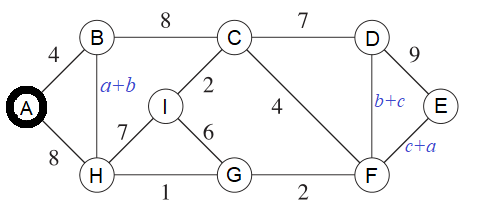
\includegraphics[width=3in]{assignment15-mst-prim/problem-graph.png}}
\caption{\label{fig:problem-graph} Graph diagram}
\end{figure}



\vspace{10pt}
{\bf (A)} Redraw the graph Figure~\ref{fig:problem-graph},
replace the edge weights $a+b$, $b+c$ and $c+a$ by the from your Student ID). 
Vertex $A$ will be your source vertex. 


\vspace{10pt}
{\bf (B)} Draw $9$ copies of the graph (no need to rewrite
the edge weights all the time \textendash{} just keep them before your eyes
as you run the Prim's algorithm). 
Show how the Prim's MST (Minimum Spanning Tree grows) one edge at a time. 
Highlight the edges selected for MST (make them bold or color them differently).
The first graph in this sequence contains no selected edges of MST, but 
the last graph in this sequence contains the full MST.
(Goodrich2011, p.652) contains sample pictures how to run the Prim's algorithm.

\vspace{10pt}
{\bf (C)} Add up the total weight of the obtained MST and 
write this in your answer (it should be the minimum value among all the
possible spanning trees in this graph). 

\end{document}

